%!TEX root = ./main.tex
La manera en la que nombramos los elementos de $\tilde{B}_n$ nos invita a pensar que habrá una clara relación entre los automorfismos $\tilde{\sigma}_i$ y los $\sigma_i$, y resulta que si la hay, y como ya es costumbre en este documento nos da una nueva equivalencia
\begin{theorem}
    La función que enviá $\sigma_i\mapsto \tilde{\sigma}_i $ define un isomorfismo de grupos entre $B_n$ y $\tilde{B}_n$
\end{theorem}
Si bien esta puede resultar interesante desde un punto de vista algebraico, nos interesa mas ver que tiene esto que ver con el Mapping Class Group de manera breve.\\

Sea $n\geq 1$, definimos $Q_n=\{(1,0),\ldots,(n,0)\}$. Sea $D$ un disco en $\R^2$ que contenga a $Q_n$ en su interior y lo orientamos en sentido contrario a las manecillas del reloj. y definimos los arcos
$$\alpha_i=[i,i+1]\times\{0\}$$
para $i=1,\ldots,n-1.$ como se puede ver en la siguiente imagen
\begin{center}
     

\tikzset{every picture/.style={line width=0.75pt}} %set default line width to 0.75pt        

\begin{tikzpicture}[x=0.75pt,y=0.75pt,yscale=-1,xscale=1]
%uncomment if require: \path (0,877); %set diagram left start at 0, and has height of 877

%Shape: Circle [id:dp37495404303702484] 
\draw   (110,145) .. controls (110,75.96) and (165.96,20) .. (235,20) .. controls (304.04,20) and (360,75.96) .. (360,145) .. controls (360,214.04) and (304.04,270) .. (235,270) .. controls (165.96,270) and (110,214.04) .. (110,145) -- cycle ;
%Straight Lines [id:da09124629345358082] 
\draw    (130,150) -- (170,150) ;
%Straight Lines [id:da35678252994237136] 
\draw    (170,150) -- (210,150) ;
%Straight Lines [id:da5587533975361445] 
\draw    (250,152) -- (290,152) ;
%Straight Lines [id:da14803740874356064] 
\draw    (290,152) -- (330,152) ;

% Text Node
\draw (142,130.4) node [anchor=north west][inner sep=0.75pt]    {$\alpha _{1}$};
% Text Node
\draw (181,130.4) node [anchor=north west][inner sep=0.75pt]    {$\alpha _{2}$};
% Text Node
\draw (221,136.4) node [anchor=north west][inner sep=0.75pt]    {$\dotsc $};
% Text Node
\draw (262,132.4) node [anchor=north west][inner sep=0.75pt]    {$\alpha _{n-2}$};
% Text Node
\draw (301,132.4) node [anchor=north west][inner sep=0.75pt]    {$\alpha _{n-1}$};
% Text Node
\draw (118,154.4) node [anchor=north west][inner sep=0.75pt]  [font=\tiny]  {$( 1,0)$};
% Text Node
\draw (159,155.4) node [anchor=north west][inner sep=0.75pt]  [font=\tiny]  {$( 2,0)$};
% Text Node
\draw (280,158.4) node [anchor=north west][inner sep=0.75pt]  [font=\tiny]  {$( n-1,0)$};
% Text Node
\draw (321,157.4) node [anchor=north west][inner sep=0.75pt]  [font=\tiny]  {$( n,0)$};


\end{tikzpicture}

 \end{center} 
 Note que por las propiedades dadas previamente $\tau_{\alpha_i}\in\mathcal{M}(D,Q_n)$ y ademas satisfacen las relaciones de trenzas, luego por \ref{homoexis} existe un homomorfismo de grupos que enviá $\sigma_i\to\tau_{\alpha_i}$, Ahora intentaremos definir un homomorfismo de grupos $\rho\colon \mathcal{M}(D,Q_n)\to \tilde{B}_n$, sabemos que escogiendo $d\in\partial D$, el grupo fundamental $\pi_1(D-Q_n,d)\cong F_n$ generado por los lazos abajo
 \begin{center}
     

\tikzset{every picture/.style={line width=0.75pt}} %set default line width to 0.75pt        

\begin{tikzpicture}[x=0.75pt,y=0.75pt,yscale=-1,xscale=1]
%uncomment if require: \path (0,877); %set diagram left start at 0, and has height of 877

%Shape: Circle [id:dp37495404303702484] 
\draw   (110,145) .. controls (110,75.96) and (165.96,20) .. (235,20) .. controls (304.04,20) and (360,75.96) .. (360,145) .. controls (360,214.04) and (304.04,270) .. (235,270) .. controls (165.96,270) and (110,214.04) .. (110,145) -- cycle ;
%Curve Lines [id:da24230856466474449] 
\draw    (230,270) .. controls (105,12.5) and (75.5,189) .. (227,270) ;
\draw [shift={(227,270)}, rotate = 208.13] [color={rgb, 255:red, 0; green, 0; blue, 0 }  ][line width=0.75]    (10.93,-3.29) .. controls (6.95,-1.4) and (3.31,-0.3) .. (0,0) .. controls (3.31,0.3) and (6.95,1.4) .. (10.93,3.29)   ;
%Curve Lines [id:da3024014633497575] 
\draw    (230,270) .. controls (302,16) and (188,131.5) .. (227,270) ;
\draw [shift={(227,270)}, rotate = 254.27] [color={rgb, 255:red, 0; green, 0; blue, 0 }  ][line width=0.75]    (10.93,-3.29) .. controls (6.95,-1.4) and (3.31,-0.3) .. (0,0) .. controls (3.31,0.3) and (6.95,1.4) .. (10.93,3.29)   ;
%Curve Lines [id:da03668887248571462] 
\draw    (230,270) .. controls (467,59.5) and (289.5,92.5) .. (227,270) ;
\draw [shift={(227,270)}, rotate = 289.4] [color={rgb, 255:red, 0; green, 0; blue, 0 }  ][line width=0.75]    (10.93,-3.29) .. controls (6.95,-1.4) and (3.31,-0.3) .. (0,0) .. controls (3.31,0.3) and (6.95,1.4) .. (10.93,3.29)   ;

% Text Node
\draw (129,152.4) node [anchor=north west][inner sep=0.75pt]  [font=\tiny]  {$( 1,0)$};
% Text Node
\draw (311,152.4) node [anchor=north west][inner sep=0.75pt]  [font=\tiny]  {$( n,0)$};
% Text Node
\draw (229,152.4) node [anchor=north west][inner sep=0.75pt]  [font=\tiny]  {$( k,0)$};
% Text Node
\draw (227,272.4) node [anchor=north west][inner sep=0.75pt]    {$d$};
% Text Node
\draw (180,142.4) node [anchor=north west][inner sep=0.75pt]    {$\cdots $};
% Text Node
\draw (260,142.4) node [anchor=north west][inner sep=0.75pt]    {$\cdots $};
% Text Node
\draw (151,122.4) node [anchor=north west][inner sep=0.75pt]    {$x_{1}$};
% Text Node
\draw (231,92.4) node [anchor=north west][inner sep=0.75pt]    {$x_{k}$};
% Text Node
\draw (321,102.4) node [anchor=north west][inner sep=0.75pt]    {$x_{n}$};


\end{tikzpicture}
 \end{center}
 Note que cada auto homeomorfismo se puede restringir a $D-Q_n$, y como por hipótesis $d$ queda fijo, por lo que induce un automorfismo $\rho(f)$, resulta que este automorfismo es un automorfismo de trenzas por lo que tenemos el siguiente teorema que nos da la ultima equivalencia
 \begin{theorem}
     Para $n\geq 1$, los homomorfismos $\eta,\rho$ son isomorfismos que hacen que el siguiente diagrama conmute
     \begin{center}
         

\tikzset{every picture/.style={line width=0.75pt}} %set default line width to 0.75pt        

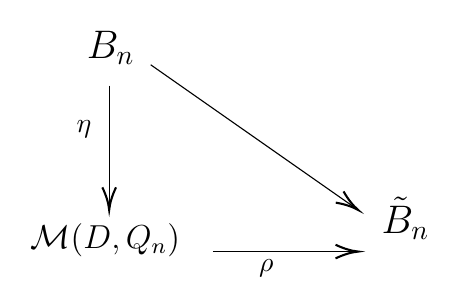
\begin{tikzpicture}[x=0.75pt,y=0.75pt,yscale=-1,xscale=1]
%uncomment if require: \path (0,877); %set diagram left start at 0, and has height of 877

%Straight Lines [id:da3495190020906457] 
\draw    (190,130) -- (190,188) ;
\draw [shift={(190,190)}, rotate = 270] [color={rgb, 255:red, 0; green, 0; blue, 0 }  ][line width=0.75]    (10.93,-3.29) .. controls (6.95,-1.4) and (3.31,-0.3) .. (0,0) .. controls (3.31,0.3) and (6.95,1.4) .. (10.93,3.29)   ;
%Straight Lines [id:da11668079361738581] 
\draw    (210,120) -- (308.36,188.85) ;
\draw [shift={(310,190)}, rotate = 214.99] [color={rgb, 255:red, 0; green, 0; blue, 0 }  ][line width=0.75]    (10.93,-3.29) .. controls (6.95,-1.4) and (3.31,-0.3) .. (0,0) .. controls (3.31,0.3) and (6.95,1.4) .. (10.93,3.29)   ;
%Straight Lines [id:da13478561325303762] 
\draw    (240,210) -- (308,210) ;
\draw [shift={(310,210)}, rotate = 180] [color={rgb, 255:red, 0; green, 0; blue, 0 }  ][line width=0.75]    (10.93,-3.29) .. controls (6.95,-1.4) and (3.31,-0.3) .. (0,0) .. controls (3.31,0.3) and (6.95,1.4) .. (10.93,3.29)   ;

% Text Node
\draw (178,102.4) node [anchor=north west][inner sep=0.75pt]  [font=\Large]  {$B_{n}$};
% Text Node
\draw (151,195.4) node [anchor=north west][inner sep=0.75pt]  [font=\large]  {$\mathcal{M}( D,Q_{n})$};
% Text Node
\draw (320,182.4) node [anchor=north west][inner sep=0.75pt]  [font=\Large]  {$\tilde{B}_{n}$};
% Text Node
\draw (261,212.4) node [anchor=north west][inner sep=0.75pt]    {$\rho $};
% Text Node
\draw (173,145.4) node [anchor=north west][inner sep=0.75pt]    {$\eta $};


\end{tikzpicture}
     \end{center}
 \end{theorem}